\documentclass{article}

\usepackage{graphicx}
\usepackage{tikz}
\usepackage{tikzsymbols}
\usetikzlibrary{calc,patterns,shapes.geometric}
\pagestyle{empty}
\usepackage[margin=0pt]{geometry}
\geometry{papersize={14in,12in}}

\def\centerarc[#1](#2)(#3:#4:#5){\draw[#1] ($(#2)+({#5*cos(#3)},{#5*sin(#3)})$) arc (#3:#4:#5);}

\begin{document}
	\begin{figure}
		\centering
		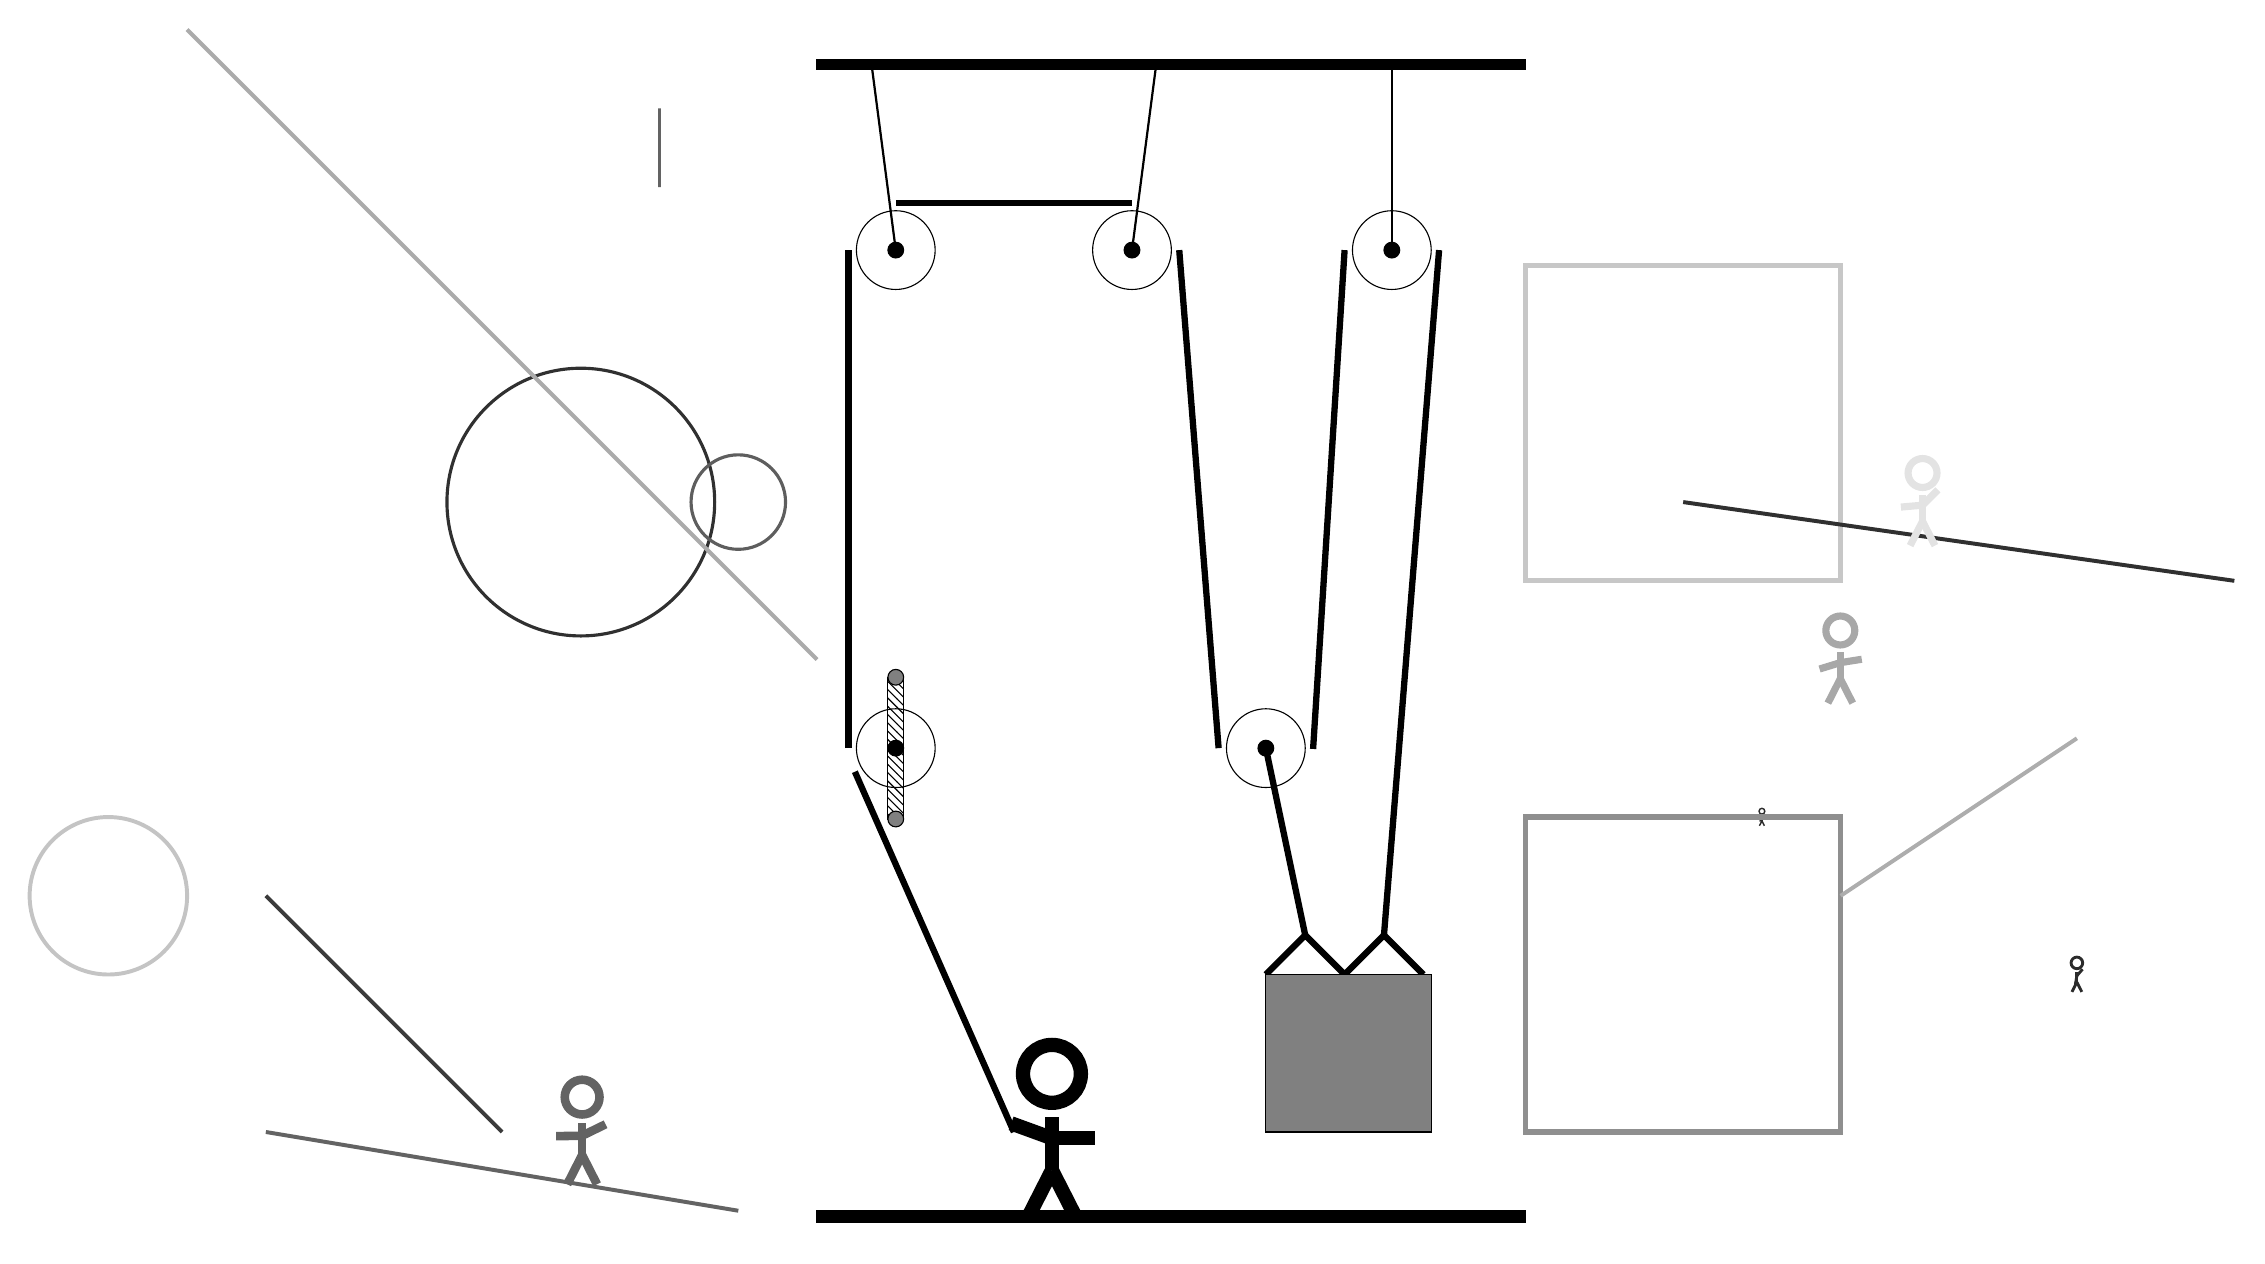
\begin{tikzpicture}
			%%%%% START %%%%%
			
			\draw[fill=black] (-3, 11.5) rectangle (6, 11.625);
			
			\draw (1, 9.2) circle (0.5);
			\draw[fill=black] (1, 9.2) circle (0.1);
			\draw[thick] (1, 9.2) -- (1.3, 11.5);
			
			\draw (4.3, 9.2) circle (0.5);
			\draw[fill=black] (4.3, 9.2) circle (0.1);
			\draw[thick] (4.3, 9.2) -- (4.3, 11.5);
			
			\draw (2.7, 2.875) circle (0.5);
			\draw[fill=black] (2.7, 2.875) circle (0.1);
			
			\draw[line width=0.8mm]  (2.7, 0.0) -- (3.2, 0.5) -- (3.7, 0.0) -- (4.2, 0.5) -- (4.7, 0.0);
			\draw[fill=black!50] (2.7, 0.0) rectangle (4.8, -2.0);
			
			\draw (-2, 9.2) circle (0.5);
			\draw[fill=black] (-2, 9.2) circle (0.1);
			\draw[thick] (-2, 9.2) -- (-2.3, 11.5);
			
			\draw[line width=0.6mm, color=black!22] (6, 5) rectangle (10, 9);
			
			\node[line width=0.2mm, color=black!83] at (13, 0) {\Strichmaxerl[2][80][49]};
			\node[line width=0.6mm, color=black!83] at (9, 2) {\Strichmaxerl[1][61][51]};
			\draw[line width=0.5mm, color=black!81](8, 6) -- (15, 5);
			\draw [line width=0.4mm, color=black!81](-6, 6) circle (1.7);
			\node[line width=0.2mm, color=black!34] at (10, 4) {\Strichmaxerl[5][17][9]};
			\draw[line width=0.5mm, color=black!61](-4, -3) -- (-10, -2);
			\draw[line width=0.7mm, color=black!44] (6, 2) rectangle (10, -2);
			\node[line width=0.7mm, color=black!61] at (-6, -2) {\Strichmaxerl[6][1][26]};
			\draw[line width=0.5mm, color=black!33](-3, 4) -- (-11, 12);
			\draw [line width=0.5mm, color=black!23](-12, 1) circle (1.0);
			\draw [line width=0.4mm, color=black!62](-7, 3) circle (0.0);
			\draw[line width=0.4mm, color=black!61] (-5, 10) rectangle (-5, 11);
			
			\draw[line width=0.5mm, color=black!77](-7, -2) -- (-10, 1);
			\draw [line width=0.4mm, color=black!63](-4, 6) circle (0.6);
			\draw[line width=0.5mm, color=black!32](10, 1) -- (13, 3);
			
			\node[line width=0.7mm, color=black!11] at (11, 6) {\Strichmaxerl[5][5][45]};
			
			\draw (-2, 2.875) circle (0.5);
			\draw[fill=black] (-2, 2.875) circle (0.1);
			\draw[pattern=north west lines, pattern color=black] (-2.1, 3.775) rectangle (-1.9, 1.975);
			\draw[fill=black!50] (-2, 3.775) circle (0.1);
			\draw[fill=black!50] (-2, 1.975) circle (0.1);
			
			\draw[line width=0.8mm](-0.5, -2) -- (-2.5196, 2.575);
			\centerarc[line width=0.8mm](-2, 2.875)(180:210:0.6);
			\draw[line width=0.8mm](-2.6, 2.875) -- (-2.6, 9.2);
			\centerarc[line width=0.8mm](-2, 9.2)(90:180:0.6);
			
			\draw[line width=0.8mm](-2, 9.8) -- (1, 9.8);
			\centerarc[line width=0.8mm](1, 9.2)(0:90:0.6);
			\draw[line width=0.8mm](1.6, 9.2) -- (2.1, 2.875);
			\centerarc[line width=0.8mm](2.7, 2.875)(180:370:0.6);
			\draw[line width=0.8mm] (3.3, 2.865) -- (3.7, 9.2);
			\centerarc[line width=0.8mm](4.3, 9.2)(0:180:0.6);
			\draw[line width=0.8mm](4.2, 0.5) -- (4.9, 9.2);
			\draw[line width=0.8mm] (3.2, 0.5) -- (2.7, 2.875);
			
			\node at (0, -2) {\Strichmaxerl[10][-20][0]};
			
			\draw[fill=black] (-3, -3) rectangle (6, -3.15);
			
			%%%%% END %%%%%
		\end{tikzpicture}
	\end{figure}	
\end{document}